\documentclass[a4paper,12pt]{article} % czcionka 10pt
\usepackage[utf8]{inputenc}
\usepackage[T1]{fontenc}
\usepackage[polish]{babel}
\usepackage{graphicx}
\usepackage{geometry}
\usepackage{fancyhdr}
\usepackage{titlesec}
\usepackage{setspace}
\usepackage{amsmath}
\usepackage{float}
\usepackage{tocloft}
\usepackage[backend=biber,sorting=none]{biblatex}
\addbibresource{../../resources.bib}

\usepackage{caption}
\captionsetup[table]{justification=raggedright, singlelinecheck=false, font=small}

% Czcionka Times New Roman
\usepackage{mathptmx}

% Marginesy 2 cm
\geometry{top=2cm,bottom=2cm,left=2cm,right=2cm}

% Interlinia
\setstretch{1.5}

% Nagłówki sekcji - odstępy 12pt przed i 6pt po nagłówku
\titlespacing*{\section}{0pt}{12pt}{6pt}
\titlespacing*{\subsection}{0pt}{12pt}{6pt}
\titlespacing*{\subsubsection}{0pt}{12pt}{6pt}

% Formatowanie nagłówków sekcji (czcionka 12pt, odpowiednie pogrubienie/kursywa)
\titleformat{\section}{\normalfont\fontsize{12}{18}\bfseries}{\thesection.}{1em}{}
\titleformat{\subsection}{\normalfont\fontsize{12}{18}\bfseries}{\thesubsection.}{1em}{}
\titleformat{\subsubsection}{\normalfont\fontsize{12}{18}\itshape}{\thesubsubsection.}{1em}{}
\titleformat{\paragraph}[hang]{\normalfont\fontsize{12}{18}\itshape}{}{0pt}{}

% Stopka - numeracja stron + imię autora
\pagestyle{fancy}
\fancyhf{}
\fancyfoot[C]{\studentName \hfill Strona \thepage}
\renewcommand{\headrulewidth}{0pt}
\renewcommand{\footrulewidth}{0.4pt}

% Tabele - automatyczne dopasowanie szerokości i odstępów
\usepackage{array}
\usepackage{booktabs}
\usepackage{longtable}
\usepackage{tabularx}
\renewcommand\tabularxcolumn[1]{>{\centering\arraybackslash}m{#1}}
\setlength{\extrarowheight}{2pt} % dodatkowa wysokość wierszy
\renewcommand{\arraystretch}{1.0} % odstęp między wierszami tabeli

%Wykresy
\captionsetup[figure]{justification=centering}

% User-fillable fields
\newcommand{\rTitle}{Badanie procesów stochastycznych}
\newcommand{\studentName}{Kacper Śmieżewski, Mikołaj Suszek}
\newcommand{\faculty}{FTiMS}
\newcommand{\fieldOfStudy}{Fizyka Techniczna}
\newcommand{\raportDate}{06/11/2026}

\begin{document}
    \begin{flushright}
    Gdańsk, \raportDate
    \end{flushright}
    \vspace{12pt}
    \textbf{\rTitle}\\
    \begin{flushleft}
      \textit{\studentName}\\
      Politechnika Gdańska,\\
      \faculty,\\ 
      \fieldOfStudy
    \end{flushleft}
\vspace{24pt}

%\renewcommand{\thesection}{\Roman{section}}
\renewcommand{\thesection}{\Roman{section}}
\addtolength{\cftsecnumwidth}{1em}

\begin{abstract}
Celem doświadczenia było zbadanie stochastycznego 
  charakteru promieniowania tła.
  Poddano analizie próbę 200 pomiarów promieniowania $\gamma$,
  z których każdy trwał 7 sekund.

  Na podstawie zebranych danych wyznaczono wartość średnią
  oraz wariancję, a następnie za pomocą
  testu statystycznego $\chi^2 = 6.1360$ zweryfikowano hipotezę 
  o zgodności otrzymanego rozkładu empirycznego
  z teoretycznym rozkładem Poissona.
\end{abstract}

\section{Cel ćwiczenia}
Celem ćwiczenia jest zapoznanie się z charakterem procesów rozpadu
promieniotwórczego.
Zjawisko to analizowane jest pod kątem fluktuacji statystycznych,
a zebrane wyniki weryfikowane są z użyciem modelu Poissona
oraz oceny zgodności testem $\chi^2$.

\section{Wstęp teoretyczny}
Rozpad promieniotwórczy jest procesem stochastycznym, 
w którym moment rozpadu danego jądra atomowego jest niemożliwy
do precyzyjnego ustalenia, a opisuje go jedynie prawdopodobieństwo.
Podstawowe prawo rozpadu promieniotwórczego określa się wzorem\cite{fw}:

\begin{equation}
N = N_0 e^{-\lambda t}
\end{equation}

gdzie $N_0$ to początkowa liczba jąder radioizotopu,
a $\lambda$ to stała rozpadu.
Różniczkując to równanie po czasie, uzyskujemy aktywność,
czyli liczbę rozpadów zachodzących w jednostce czasu:
\begin{equation}
\frac{dN}{dt} = -\lambda N_0 e^{-\lambda t} = -\lambda N
\end{equation}

W przypadku badania tła, gdzie prawdopodobieństwo rejestracji zdarzenia w krótkim oknie pomiarowym jest bardzo małe, 
rozkład fluktuacji opisywany jest funkcją prawdopodobieństwa Poissona\cite{erroranal}:
\begin{equation}
P(n) = \frac{m^n}{n!} e^{-m}
\end{equation}
gdzie $n$ to liczba zliczeń w przedziale czasu, a $m$ to wartość średnia. 
Zgodność zebranych danych doświadczalnych z teorią weryfikuje się sumą względnych odchyleń kwadratowych określaną jako statystyka $\chi^2$:

\begin{equation}
\chi^2 = \sum \frac{(\upsilon_i - nP_i)^2}{nP_i}
\end{equation}

\section{Przebieg pomiarów}
Licznikiem impulsów mierzono ilość zliczeń cząstek $\gamma$
przez 7s na pomiar. 

\section{Wyniki i dyskusja}
Zebrane dane z 200 pomiarów tła podzielono na
8 dyskretnych przedziałów (od 0 do 7 zarejestrowanych zliczeń).
Wyznaczona średnia empiryczna wynosi $m = 2.64$, podczas gdy obliczona z próby wariancja to $\sigma^2 \approx 2.23$.

W oparciu o średnią $m$ oraz całkowitą ilość pomiarów $N = 200$,
wyliczono teoretyczne prawdopodobieństwa $P_i$ 
oraz oczekiwaną liczbę wystąpień $nP_i$ dla każdego ze stanów.
Zestawienie tych wartości wraz ze składnikami testu statystycznego
zaprezentowano w Tabeli \ref{tab:dist}.

\begin{table}[H]
  \centering
  \caption{Zestawienie wyników pomiarów i obliczeń dla rozkładu Poissona}
  \label{tab:dist}
  \begin{tabular}{ccccc} 
\midrule
\begin{tabular}[c]{@{}c@{}}liczba\\~zliczeń\end{tabular} & \begin{tabular}[c]{@{}c@{}}rozkład\\~doświadczalny\end{tabular} & \begin{tabular}[c]{@{}c@{}}prawdopodobieństwo~\\Poissona\end{tabular} & \begin{tabular}[c]{@{}c@{}}rozkład\\~teoretyczny\end{tabular} & \begin{tabular}[c]{@{}c@{}}względne odchylenie\\~kwadratów\end{tabular}  \\ 
\midrule
0                                                        & 14                                                              & 0.071361                                                              & 14.27225                                                      & 0.0052                                                                   \\
1                                                        & 29                                                              & 0.188394                                                              & 37.67875                                                      & 1.9990                                                                   \\
2                                                        & 57                                                              & 0.248680                                                              & 49.73595                                                      & 1.0609                                                                   \\
3                                                        & 49                                                              & 0.218838                                                              & 43.76764                                                      & 0.6255                                                                   \\
4                                                        & 25                                                              & 0.144433                                                              & 28.88664                                                      & 0.5229                                                                   \\
5                                                        & 19                                                              & 0.076261                                                              & 15.25215                                                      & 0.9209                                                                   \\
6                                                        & 6                                                               & 0.033555                                                              & 06.71094                                                      & 0.0753                                                                   \\
7                                                        & 1                                                               & 0.012655                                                              & 02.53099                                                      & 0.9261                                                                   \\
\midrule
\end{tabular}

\end{table}

Sumując wartości względnych odchyleń kwadratowych,
uzyskano statystykę próby równą $\chi^2 = 6.136$.
Przyjęto standardowy poziom istotności na poziomie $\alpha = 0.05$.
Ze względu na podział danych na 8 klas 
oraz konieczność estymacji z próby jednego parametru
(wartości średniej), wyznaczono $k = 6$ stopni swobody. 

Wartość krytyczna odczytana z tablic rozkładu 
wynosi $\chi^2_{kryt} = 12.592$ \cite{fw}. 
Wyliczona wartość doświadczalna jest mniejsza 
od granicy odrzucenia,
a dokładne $p-value$ testu wynosi 0.408.
Nie ma więc podstaw do odrzucenia hipotezy.

Dopasowanie przedstawiono na Rysunku \ref{plot}.
Rozkład doświadczalny w dużej mierze pokrywa się z wartościami przewidywanymi przez model Poissona.

\begin{figure}[H]
  \centering
  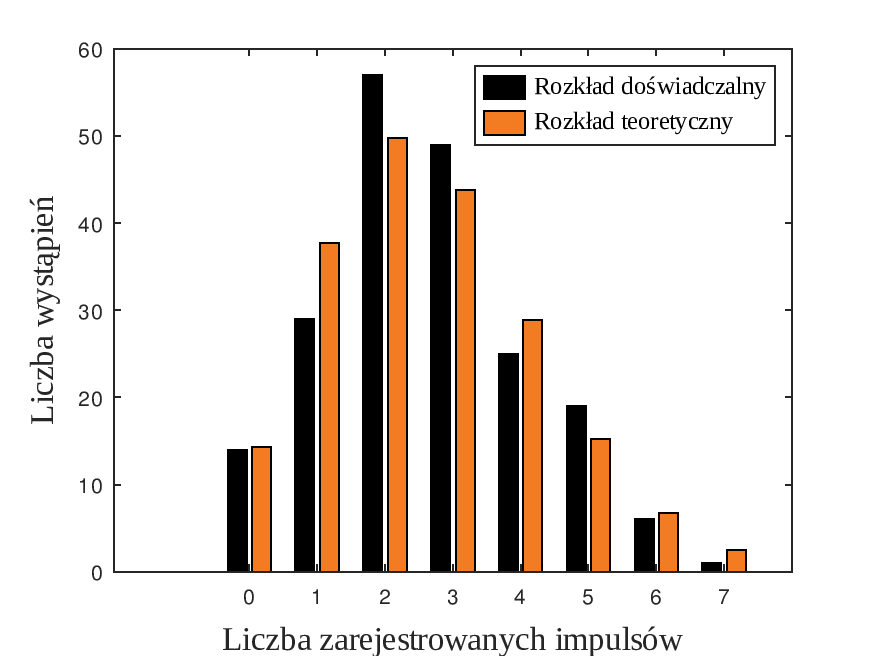
\includegraphics[width=12cm]{fig.png}
  \caption{Porównanie pomiarów promieniowania tła z teoretycznym modelem Poissona}
  \label{plot}
\end{figure}

\section{Wnioski}
\begin{enumerate}
    \item \textbf{Stochastyczny charakter zjawiska:} Potwierdzono, że występowanie promieniowania tła w otoczeniu laboratoryjnym przejawia silne odchylenia.
    \item \textbf{Zgodność parametrów rozkładu:} Wyznaczona z próby średnia ($m = 2.64$) oraz wariancja ($\sigma^2 \approx 2.23$) przyjmują bardzo zbliżone wartości.
      Równość tych dwóch parametrów jest jedną z fundamentalnych cech rozkładu Poissona,
      co wstępnie potwierdza słuszność przyjętego modelu fizycznego.
    \item \textbf{Weryfikacja testem statystycznym:} 
      Ilościowa analiza zbieżności wykazała brak istotnych rozbieżności pomiędzy uzyskanym rozkładem empirycznym a założonym modelem teoretycznym.
      Otrzymana statystyka $\chi^2 \approx 6.136$ pozwoliła na zaakceptowanie hipotezy o zgodności fluktuacji z rozkładem Poissona na poziomie istotności $\alpha = 0.05$.
\end{enumerate}

\end{document}
